\newcommand{\Pythia}{\textsc{Pythia6}}
\newcommand{\Pythiaeight}{\textsc{Pythia8}}
\newcommand{\Powheg}{\textsc{Powheg}}
\newcommand{\Mcatnlo}{\textsc{Mc@Nlo}}
\newcommand{\Herwig}{\textsc{Herwig}}
\newcommand{\Alpgen}{\textsc{Alpgen}}
\newcommand{\Sherpa}{\textsc{Sherpa}}
\def\Zgll{\ensuremath{Z/\gamma^* \rightarrow \ell\ell}}
\def\m{\ensuremath{M}}
\def\mll{\ensuremath{\m_{\ell\ell}}}
\def\Wplusmunu {\ensuremath{\Wplus  \rightarrow \mu^+\nu}}
\def\Wminusmunu{\ensuremath{\Wminus \rightarrow \mu^-\bar{\nu}}}
\def\Wpluslnu {\ensuremath{\Wplus  \rightarrow \ell^+\nu}}
\def\Wminuslnu{\ensuremath{\Wminus \rightarrow \ell^-\bar{\nu}}}

% ANALYSIS
\slide{ Thesis topic }
{
  \begin{columns}
    \begin{column}{0.5\textwidth}
      \begin{tikzpicture}
        \begin{scope}
          [small mindmap,
          every node/.style={concept, execute at begin node=\hskip0pt, concept color=BrickRed, circular drop shadow, minimum size=1.8cm},
          every child/.style={concept color=BrickRed!100!gray!100, font=\large},
          concept/.append style={fill=BrickRed,text=white},
          grow cyclic,
          level 1/.append style={level distance=3.4cm, sibling angle=90}]
          \node [concept color=black, fill=white, text=black, minimum size=2.8cm] {7\,TeV \mbox{Inclusive W/Z} Cross~Section Measurement}[clockwise from=135]
          child [visible on=<1->] { node (Zee) {\Zee} }
          child [visible on=<1->] { node (Zmumu) {\Zmm} }
          child [visible on=<1->] { node (Wmunu) {\Wmn} }
          child [visible on=<1->] { node (Wenu) {\Wen} }
          ;
        \end{scope}
      \end{tikzpicture}

    \end{column}
    \begin{column}{0.1\textwidth}<1->
    \end{column}
    \begin{column}{0.4\textwidth}<1->
      \begin{itemize}
      \item \textit{``Measurement of differential inclusive \textbf{\W\ boson} production and decay cross sections in the muon channel using the ATLAS Detector.''}
      \item Part of the comprehensive 2011 W/Z cross-section measurement paper at ATLAS
      \item Chicago team: Anton Kapliy, Peter Onyisi, Mel Shochet
      \item 20+ collaborators, mostly in Europe
      \end{itemize}
    \end{column}
  \end{columns}

}

% SM
\slide{ W in the Standard Model }
{
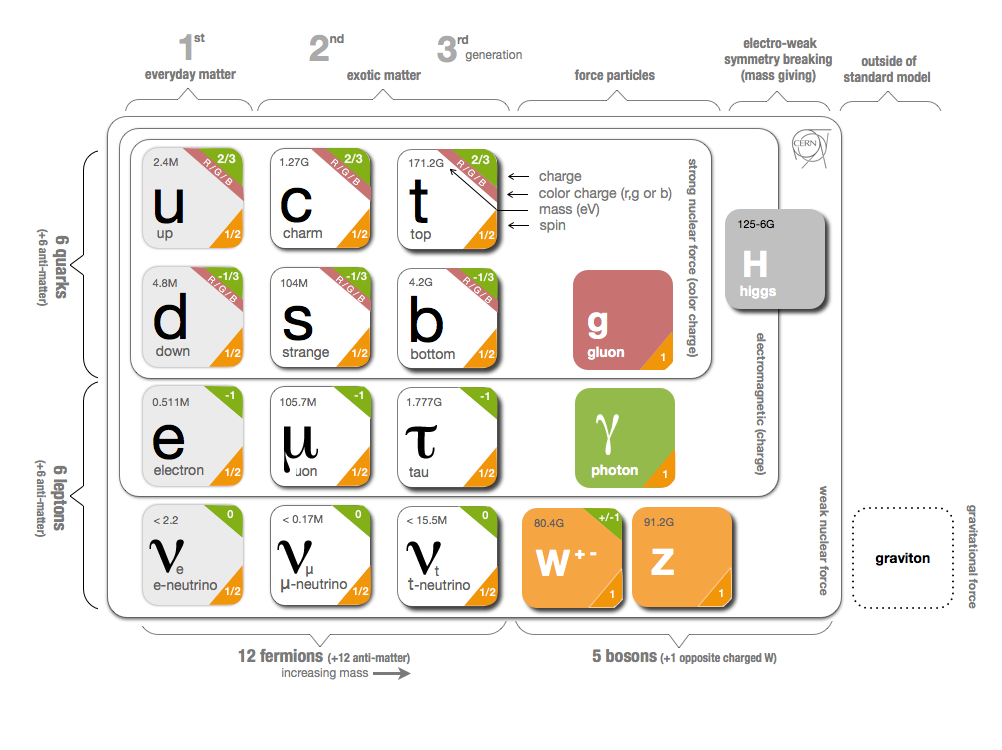
\includegraphics[width=0.8\textwidth]{dates/mtg/figures/wz/sm} \\
\textbf{$W$ boson}: mediator of charged weak currents generated from SU(2).
}

\slide{ W boson production (I) : protons }
{

\colb[T]
\column{.7\textwidth}
\centering
\iteb
\item Protons can be viewed as collections of \red{partons}:
\iteb
\item Valence quarks: Up+Up+Down
\item Sea quarks
\item Gluons
\itee
\itee
\column{.3\textwidth}
\centering
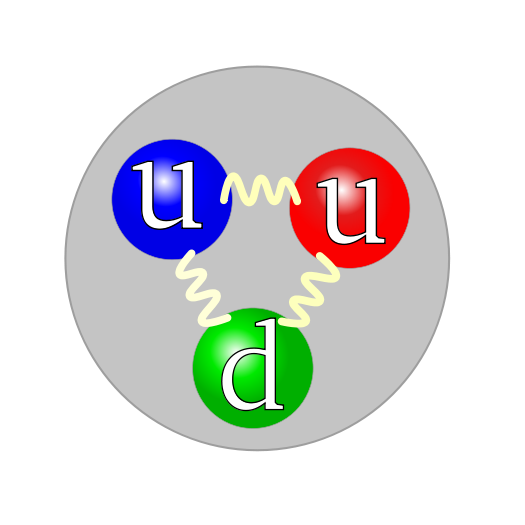
\includegraphics[width=0.5\textwidth]{dates/mtg/figures/wz/proton}
\cole

\vspace{.3cm}
W bosons are produced when two partons interact: \\
\centering
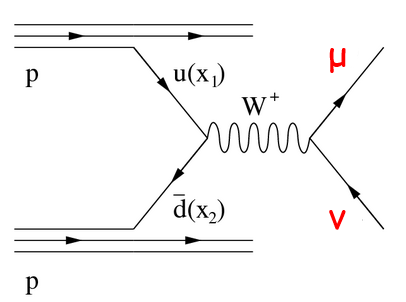
\includegraphics[width=0.4\textwidth]{dates/mtg/figures/wz/wmunuf} 

}

\def\sighat{\hat{\sigma}}
\slide{ W boson production (II) : factorization}
{

\colb[T]
\column{.65\textwidth}
\centering
Cross-section according to factorization theorem:
\iteb
\item Parton-parton hard scatter vertex $\sighat$ (perturbative QCD)
\item Momentum fraction $x$ carried by each parton (empirical PDFs)
\itee
\column{.35\textwidth}
\centering
\includegraphics[width=0.7\textwidth]{/home/antonk/thesis/tex/theory/fig/Hardscattering}
\cole

\begin{equation}
\begin{split}
\sigma_{AB\to W} = \sum\limits_{partons} \int dx_a dx_b\; f_{a/A}(x_a,\mu_{F}^2) f_{b/B}(x_b,\mu_{F}^2) \cdot \\
\left[ \sighat_{LO}(x_{a}x_{b}s) + \alpha_{s}(\mu_{R}^2)\sighat_{NLO}(x_{a}x_{b}s) + \left(\alpha_{s}(\mu_{R}^2)\right)^{2}\sighat_{NNLO}(x_{a}x_{b}s) + \ldots \right]
\end{split}
\end{equation}

\centering
\tiny{ Example: process at the next-to-leading (NLO) order: } \\
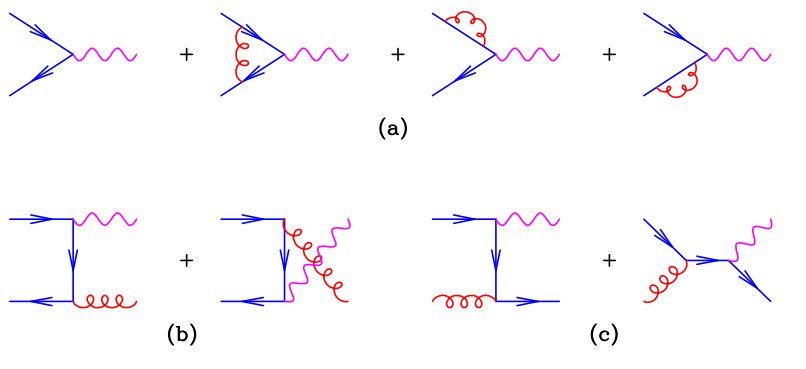
\includegraphics[width=0.45\textwidth]{dates/mtg/figures/wz/nlo}

}

\slide{ W boson production (III) : hard scatter }
{

\centering
Contributions of various $q\bar{q}$ processes at 7 TeV:

\centering
\includegraphics[width=0.40\textwidth]{/home/antonk/thesis/tex/theory/fig/Wprod}

$$ \sighat(q\bar{q'} \rightarrow W) = 2\pi|V_{qq'}|^2 \frac{G_F}{\sqrt{2}} M_{W}^{2} \cdot \delta\left(Q^2 - M_{W}^{2}\right)$$

}

\slide{ W boson production (IV) : PDFs }
{

\centering
\small{ Example PDFs at $Q^2 = 4$~GeV$^2$ and $Q^2 = 10^4$~GeV$^2$ (CT10 collaboration) }

\includegraphics[width=0.45\columnwidth]{/home/antonk/thesis/tex/theory/fig/examplepdfs_q2} 
\includegraphics[width=0.45\columnwidth]{/home/antonk/thesis/tex/theory/fig/examplepdfs_q100}

\small{PDFs can be extracted from W rapidity $y$ (boost along the beam axis from the lab frame to the frame where the boson moves only perpendicularly to the beam):}
$$ x_a = \frac{m_W}{\sqrt s} e^{y_W} $$
$$ x_b = \frac{m_W}{\sqrt s} e^{-y_W} $$

}

\slide{ W boson decay }
{
Thanks to V-A nature of weak interaction, W and muon directions are correlated.\\
$\rightarrow$ study the muon instead of the W, for which we cannot reconstruct $p_Z$.

\vspace{.2cm}
\colb[T]
\column{.70\textwidth}
Cross-section is measured in bins of:
\iteb
\item Inclusively
\item Muon $\eta$
\item Muon $\eta$ x $p_T$
\itee
\column{.30\textwidth}
\centering
\includegraphics[width=0.80\textwidth]{/home/antonk/thesis/tex/theory/fig/decay}
\cole

\vspace{.3cm}
Transverse momentum $p_T$ and pseudorapidity $\eta$:
\includegraphics[width=0.44\textwidth]{/home/antonk/thesis/tex/method/fig/PT}
\includegraphics[width=0.44\textwidth]{/home/antonk/thesis/tex/method/fig/pseudorapidity}

}

\slide{ How do we measure the cross-section? } {

\centering
\huge{
$\sigma \times BR = \frac{N - B}{C \cdot A \cdot L_{int} }$
}

\normalsize
\vspace{.3cm}
\begin{itemize}
\item $N$ - number of \Wboson\ candidate events in data
\item $B$ - number of background events
\item $L_{int}$ - integrated luminosity (total amount of collected data)
\item $C$ - corrects for detector efficiency and resolution effects. Derived from Monte-Carlo and translates the cross-sections from ``reconstruction level'' to ``generator level'', which is independent of the specific features of the detector.
\item $A$ - extrapolates cross-sections to the full phase space volume before any fiducial cuts (integrated case only)
\end{itemize}
}

\slide{ W boson: why bother? }
{
\colb[T]
\column{.6\textwidth}
\centering
\iteb
\item Proton structure
\iteb
\item Validate existing PDF predictions
\item Provide new constraints for future expt's
\item E.g., cross-section vs $\eta$ (see figure)
\itee
\item Tests of perturbative QCD
\iteb
\item Last published measurement: 2010 data
\item Achieved precision: $\mathcal{O}(2-3\%)$
\item Today, we can finally reach below 1\%
\itee
\item Better understanding of the detector
\iteb
\item People focus on Higgs, new physics
\item These analyses don't need percent-level understanding of the detector
\item We can fill the gap
\itee
\itee
\column{.4\textwidth}
\centering
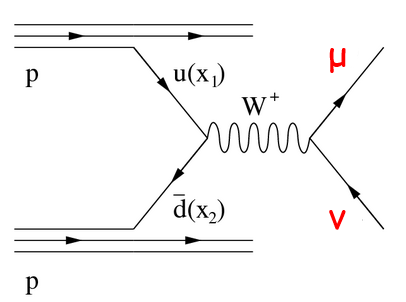
\includegraphics[width=0.6\textwidth]{dates/mtg/figures/wz/wmunuf} \\
\tiny{ Explaining pseudorapidity ($\eta$): } \\
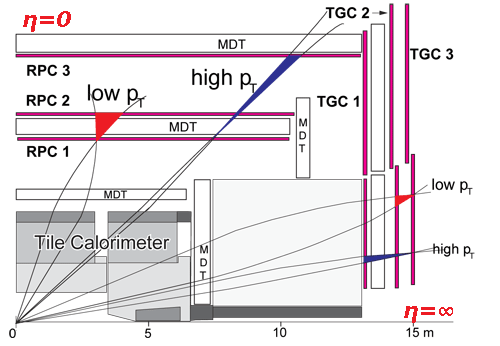
\includegraphics[width=1.0\textwidth]{dates/mtg/figures/wz/eta} \\
\cole
}

% LHC
\slide{ The Large Hadron Collider }
{
\centering
LHC: world's largest particle accelerator located at CERN (near Geneva). \\
27-km tunnel, 2011 pp collisions at 7 TeV \\
Two bunches with $10^{11}$ protons each collide every 50 ns. \\
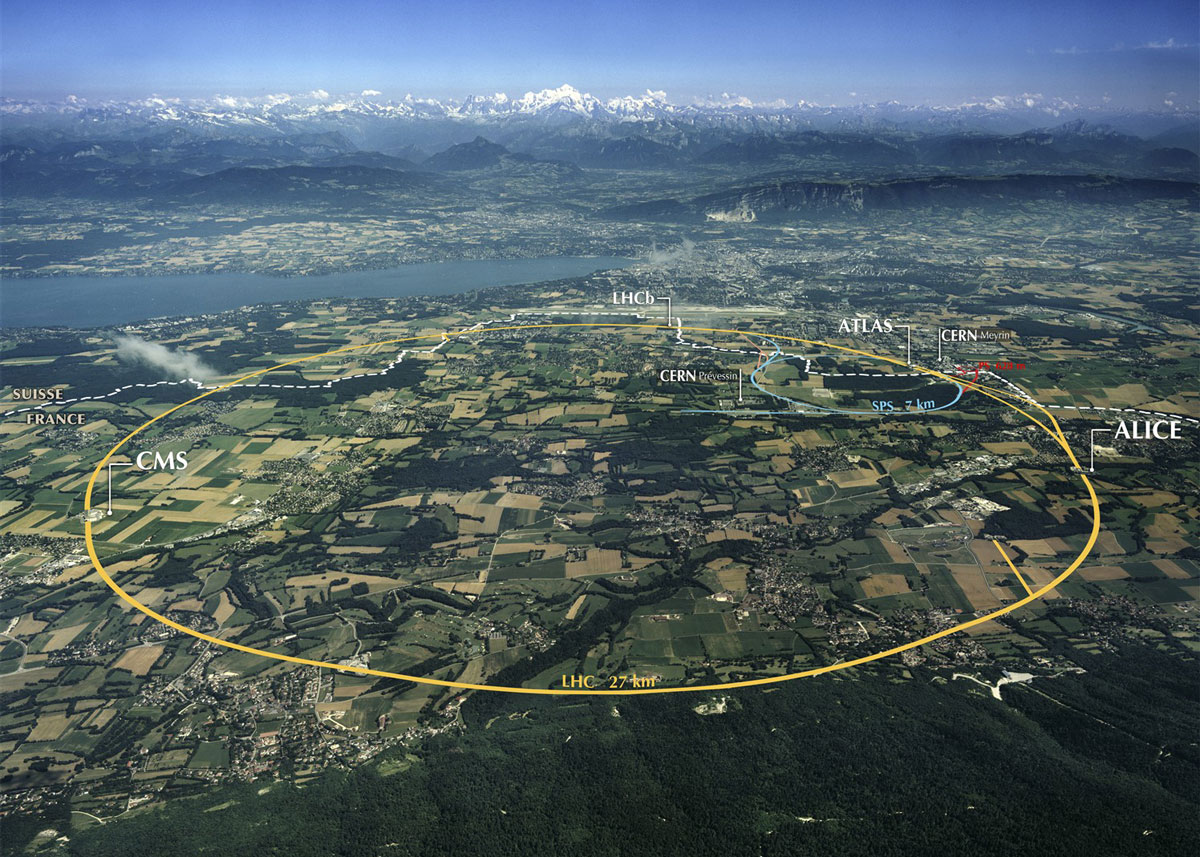
\includegraphics[width=0.8\textwidth]{dates/mtg/figures/atlas/LHC}

}

% ATLAS cavern
\slide{ ATLAS experiment: overview }
{
\centering
One of the two general-purpose experiments at LHC.\\
100 meters underground, 45 meters long, 7000 tons. \\
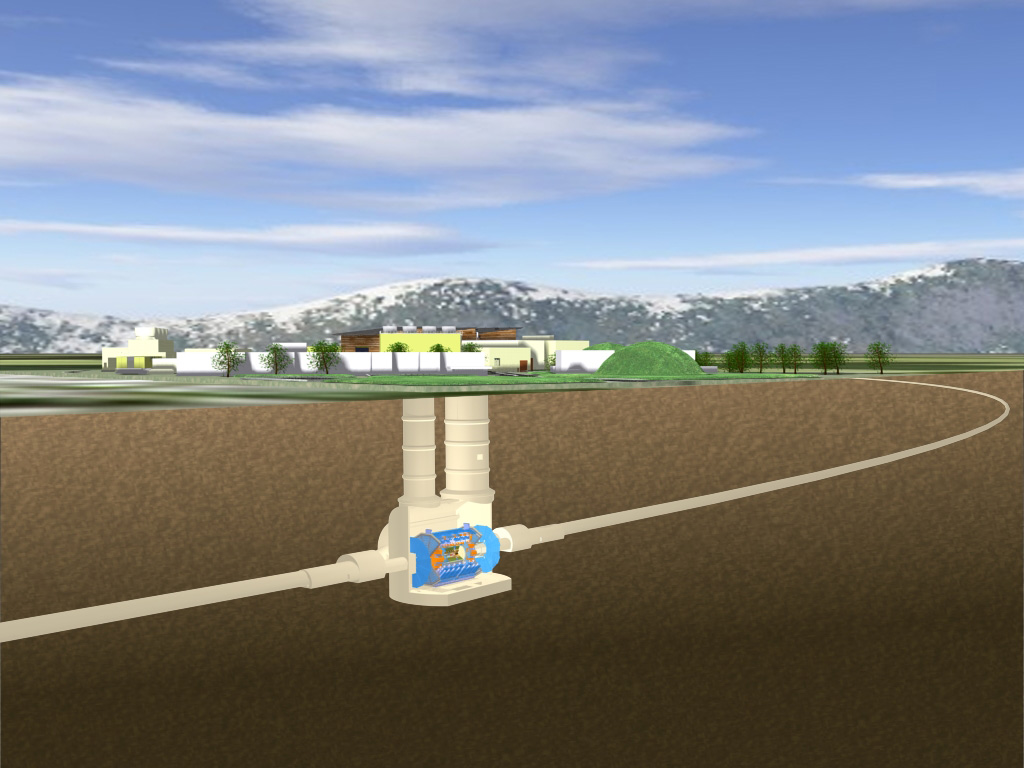
\includegraphics[width=0.8\textwidth]{dates/mtg/figures/atlas/ATLASUG}

}

% ATLAS experiment
\slide{ ATLAS experiment: details }
{
\centering
This analysis mostly relies on Inner Detector and Muon Spectrometer. \\
Calorimeters are also important to measure missing energy. \\
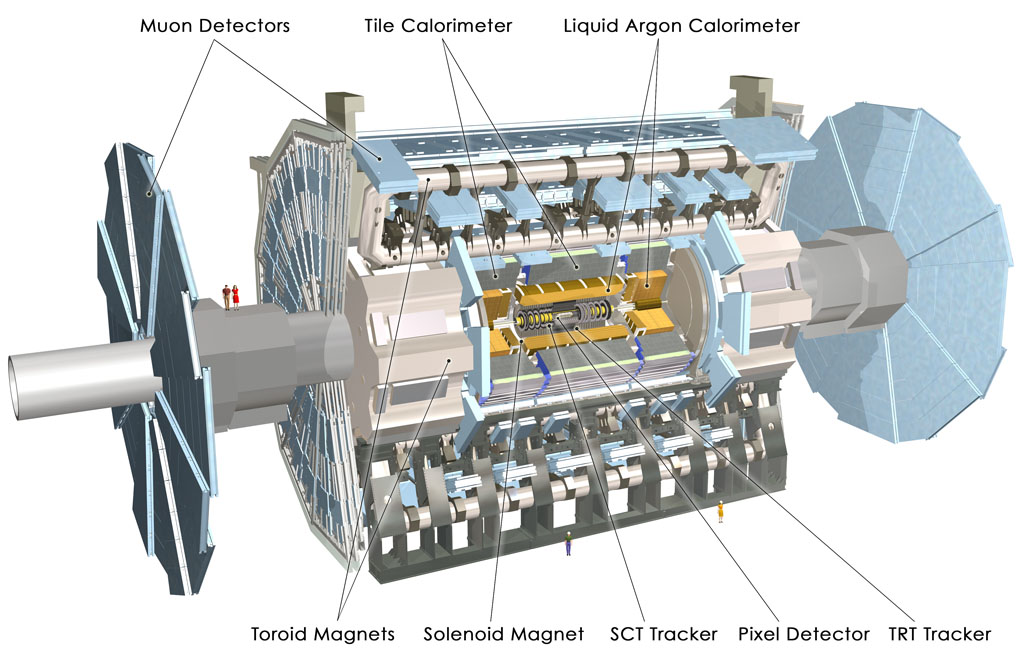
\includegraphics[width=0.8\textwidth]{dates/mtg/figures/atlas/ATLAS}

}

\slide{ $W \rightarrow \mu \nu$ in the detector }
{
\centering
\iteb
\item Muons are measured from tracker hits and muon spectrometer stations
\item Neutrinos escape undetected - but we measure ``missing energy''
\itee
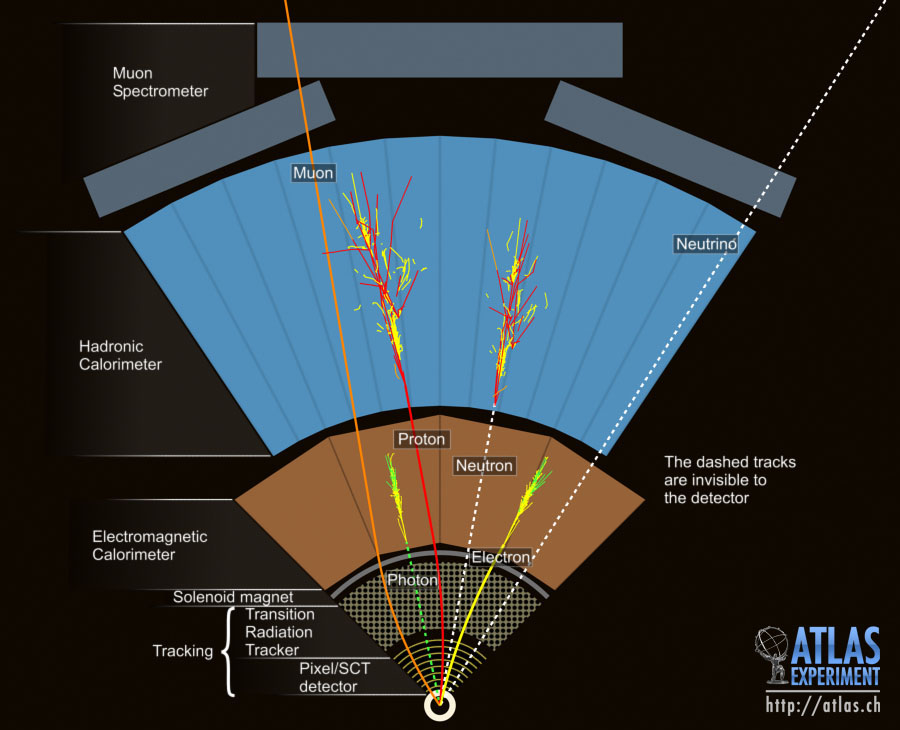
\includegraphics[width=0.7\textwidth]{dates/mtg/figures/wz/particles}

}

%%%%%%%%%%%%%%%%%%%%%%%%%%%%%%%%%%%%%%%%%%%%%%%%%%%%%
% why 2011 - pt.1
%%%%%%%%%%%%%%%%%%%%%%%%%%%%%%%%%%%%%%%%%%%%%%%%%%%%%
\begin{frame}{It's 2013. Why still use 2011 data?}
\begin{itemize}
\item All 2011 analyses used a trigger recommended by muon experts
\item We discovered disagreements in left-vs-right side of the detector
\end{itemize}

\centering
\includegraphics[width=0.4\textwidth]{/home/antonk/thesis/tex/event/AC/old/W_NOM_Q0_stack_d3_eta_lpt_met_y_2__1_z_0__1_NEG}
\includegraphics[width=0.4\textwidth]{/home/antonk/thesis/tex/event/AC/old/W_NOM_Q0_stack_d3_eta_lpt_met_y_2__1_z_0__1_POS}

~~~~~~~~~~~~~~~~~~~~~~~~~~~~~~~~~~~~~~$W^-$~~~~~~~~~~~~~~~~~~~~~~~~~~~~$W^+$
\end{frame}

% why 2011 - pt.2
\begin{frame}{It's 2013. Why still use 2011 data?}
\begin{itemize}
\item After the trigger problem was understood, we proposed a solution
\item Left-vs-right side agree within uncertainties
\end{itemize}

\centering
\includegraphics[width=0.4\textwidth]{/home/antonk/thesis/tex/event/AC/new/W_NOM_Q0_stack_d3_eta_lpt_met_y_2__1_z_0__1_NEG}
\includegraphics[width=0.4\textwidth]{/home/antonk/thesis/tex/event/AC/new/W_NOM_Q0_stack_d3_eta_lpt_met_y_2__1_z_0__1_POS}

~~~~~~~~~~~~~~~~~~~~~~~~~~~~~~~~~~~~~~$W^-$~~~~~~~~~~~~~~~~~~~~~~~~~~~~$W^+$
\end{frame}

\begin{frame}{Corrections to Monte-Carlo}
\begin{itemize}
\item Data-driven corrections to Monte-Carlo are derived via Z tag-and-probe:
\begin{itemize}
\item Muon momentum scale
\item Muon trigger,reconstruction,isolation scale factors
\end{itemize}
\item All corrections must be understood to better than a percent level!
\end{itemize}

\vspace{.3cm}
\centering
\tiny{Example: muon trigger efficiency corrections for periods G-I (left) and L3-L4 (right) } \\
\includegraphics[width=0.45\textwidth]{/home/antonk/thesis/tex/MuonPerformance/figures/scaleFactors/mu18_neg_SF_eta_pt}
\includegraphics[width=0.45\textwidth]{/home/antonk/thesis/tex/MuonPerformance/figures/scaleFactors/rpc_pos_SF_eta_pt}

\end{frame}

%  Selection
\slide{W,Z selection in muon channels}
{
Common selection:
\iteb
\item \textit{Single muon triggers}: EF\_mu18 or EF\_mu18\_medium
\item Primary vertex with $\ge$ 3 tracks
\item Reject events with $BadLooser$ jets or jets in $LarHole$ region
\item Combined STACO muons passing MCP quality cuts and $|z_0|~<~10~mm$
\item Muon kinematics: $p_T~>~25~\GeV$ and $|\eta|~<~2.4$
\item Tracking isolation: $\sum \pt(\Delta R~<~0.4) / \pt~<~0.1$
\itee
\textbf{\large $\mathbf{W \to \mu\nu}$ channel}:
\iteb
\item \textit{Exactly one isolated muon}
\item $\met > 25\,\GeV$, $\mt > 40\,\GeV$ using \texttt{MET\_RefFinal}
\itee
\textbf{\large $\mathbf{Z \to \mu\mu}$ channel}:
\iteb
\item \textit{Exactly two isolated muons}
\item Opposite charges
\item $46 < m_{\mu\mu} < 150\gev$
\itee
}

% background
\slide{Backgrounds}
{
\iteb
\item Small backgrounds from other \Zll\ and \Wln\ channels, Dibosons,
  $t\bar{t}$ and single $t$ are estimated from MCs
\iteb
\item $\Zmm$ and $\Wmn$: Powheg+Pythia, Powheg+Herwig, MCNLO
\item $\tau$ samples: Alpgen+Jimmy, rapidity-reweighted
\item dibosons: Herwig
\item top: MCNLO
\itee
\item Main work is multijet background estimation to permil level
\iteb
\item Short summary on the next slide
\itee
\itee
}

% qcd
\slide{Multi-jet background in \Wmn (I)}
{
\iteb
\item LHC produces a lot of jets
\item Heavy-flavor jets contain muons
\item Easy to mistake these for a W decay
\item Multi-jets are difficult to model in MC
\iteb
\item Data-driven fit in a control region
\item Control region defined by inverting isolation cut
\itee
\itee

\colb[T]
\column{.4\textwidth}
\centering
\small{
\vspace{.5cm}
Isolation: $p_T$-sum of all tracks within a cone of $\Delta R = 0.4$ around the muon (excluding the muon itself), divided by the muon $p_T$. Dimensionless quantity that peaks at 0 for well-isolated muons from W decay.
}
\column{.6\textwidth}
\centering
\includegraphics[width=0.8\textwidth]{/home/antonk/thesis/tex/event/fig/TEST_ISOPLOT_NEG_lepton_ptiso40r}
\cole

}

\slide{Multi-jet background in \Wmn (II)}
{
\iteb
\item Template fits vs $\met$ and $\mt$
\item Floating EWK template from MC
\iteb
\item 1D: separate fits in each $|\eta|$ bin
\item 2D: separate fits in each $p_{T}$ x $|\eta|$ bin
\item Systematics: Fit var., range, binning; pileup; anti-isolation, MC, etc
\itee
\itee

\centering
\footnotesize{Example: \Powheg\Pythia (left) vs \Mcatnlo (right) fits in the $p_T$-inclusive case:}

\includegraphics[width=0.42\textwidth]{/home/antonk/SupportingDocument/Wmunu/figures/met_shape/Q1_powheg_pythia}
\includegraphics[width=0.42\textwidth]{/home/antonk/SupportingDocument/Wmunu/figures/met_shape/Q1_mcnlo}

}

%===========================================
%  Slide -1
%===========================================

\slide{Representative fits for \Wmn\ (2D)}
{
\begin{figure}[phtb]
  \begin{center}
      \includegraphics[width=0.33\textwidth]{/home/antonk/SupportingDocument/Wmunu/figures/qcdfits/Q0_x_2_2_y_2_2}
      \includegraphics[width=0.33\textwidth]{/home/antonk/SupportingDocument/Wmunu/figures/qcdfits/Q0_x_11_11_y_2_2}

      \includegraphics[width=0.33\textwidth]{/home/antonk/SupportingDocument/Wmunu/figures/qcdfits/Q0_x_2_2_y_6_6}
      \includegraphics[width=0.33\textwidth]{/home/antonk/SupportingDocument/Wmunu/figures/qcdfits/Q0_x_11_11_y_6_6}
  \end{center}
\end{figure}
}


\slide{Summary of backgrounds in \Wmn}
{

\colb
\col{0.5}

\centering
\includegraphics[width=0.7\textwidth]{/home/antonk/SupportingDocument/Wmunu/figures/bgcomp/bgsummary_POS_pt25}

\iteb
\item EWK and QCD backgrounds are comparable in size
\item Uncertainty on QCD is much larger
\item Largest EWK backgrounds: \Wtau\ and \Zmm; top at high $p_T$
\itee

\col{0.5}

\centering
\includegraphics[width=0.7\textwidth]{/home/antonk/SupportingDocument/Wmunu/figures/bgcomp/bgsummary_NEG_pt2}

\includegraphics[width=0.7\textwidth]{/home/antonk/SupportingDocument/Wmunu/figures/bgcomp/bgsummary_NEG_pt7}

\cole

\mybox{2.4}{1.3}{\footnotesize $\mu^{+}: p_{T}>25\,GeV$}
\mybox{13.}{0.01}{\footnotesize $\mu^{-}: 25<p_{T}<30\,GeV$}
\mybox{13.}{8.9}{\footnotesize $\mu^{-}: p_{T}>50\,GeV$}

}

% stacks
\slide{Control plots} 
{
\only<1>{$\Wminus  \rightarrow \mu^-\nu$}
\only<2>{$\Wplus  \rightarrow \mu^{+} \nu$}
\scriptsize{(Systematic band includes all experimental uncertainties + MC generators + boson $p_{T}$.)}

\centering
\vspace{-.3cm}
 \begin{columns}
  \begin{column}{0.32\textwidth}
     \begin{center}
       Muon $\eta$ \\
       \vspace{-.03cm}
       \includegraphics[width=1.00\textwidth]<1>{/home/antonk/SupportingDocument/Wmunu/figures/control_plots/inclusive25/P_stack_d3_eta_lpt_met_y_2__1_z_0__1_NEG}
       \includegraphics[width=1.00\textwidth]<2>{/home/antonk/SupportingDocument/Wmunu/figures/control_plots/inclusive25/P_stack_d3_eta_lpt_met_y_2__1_z_0__1_POS}
     \end{center}
     \vspace{-.7cm}
     \begin{center}
       Muon $p_T$ \\
       \vspace{-.03cm}
       \includegraphics[width=1.00\textwidth]<1>{/home/antonk/SupportingDocument/Wmunu/figures/control_plots/inclusive25/P_stack_lpt_NEG}
       \includegraphics[width=1.00\textwidth]<2>{/home/antonk/SupportingDocument/Wmunu/figures/control_plots/inclusive25/P_stack_lpt_POS}
     \end{center}
  \end{column}

  \begin{column}{0.32\textwidth}
     \begin{center}
       $E_T^{Miss}$ \\
       \vspace{-.03cm}
       \includegraphics[width=1.00\textwidth]<1>{/home/antonk/SupportingDocument/Wmunu/figures/control_plots/inclusive25/P_stack_d3_abseta_lpt_met_x_0__1_y_2__1_NEG}
       \includegraphics[width=1.00\textwidth]<2>{/home/antonk/SupportingDocument/Wmunu/figures/control_plots/inclusive25/P_stack_d3_abseta_lpt_met_x_0__1_y_2__1_POS}
     \end{center}
     \vspace{-.7cm}
     \begin{center}
       $m_T^{W}$ \\
       \vspace{-.03cm}
       \includegraphics[width=1.00\textwidth]<1>{/home/antonk/SupportingDocument/Wmunu/figures/control_plots/inclusive25/P_stack_d3_abseta_lpt_wmt_x_0__1_y_2__1_NEG}
       \includegraphics[width=1.00\textwidth]<2>{/home/antonk/SupportingDocument/Wmunu/figures/control_plots/inclusive25/P_stack_d3_abseta_lpt_wmt_x_0__1_y_2__1_POS}
     \end{center}
  \end{column}

\end{columns}
}

% summary of uncertainties
\slide{Summary of uncertainties for \Wmn (I) }
{

\begin{table}
  \scriptsize
  \begin{center}
  \input{/home/antonk/thesis/tex/Wmunu/figures/res/Wmn_SYSTEM_0D_PT25_SUM_Unc_proj}
    \caption{Summary of the systematic uncertainties on the integrated  \Wmunum\ and \Wmunup\ cross-sections.}
  \end{center}
\end{table}

}

\slide{Summary of uncertainties for \Wmn (II) }
{

Representative uncertainties for \red{$W^-$}: $p_{T}>25$, $25<p_{T}<30$, $40<p_{T}<45$
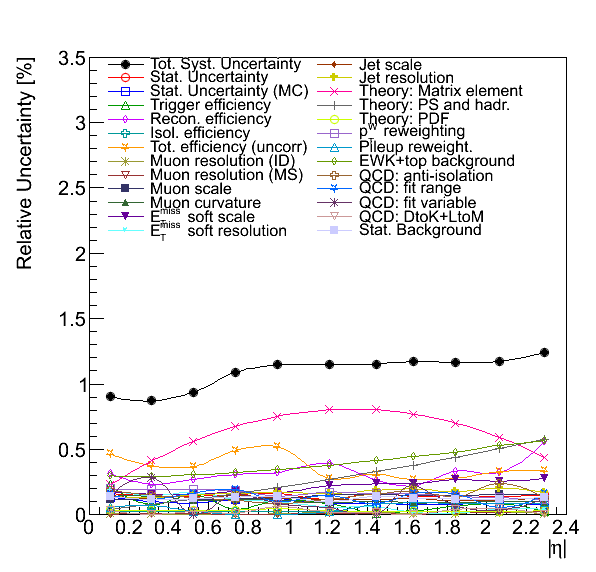
\includegraphics[width=0.32\textwidth]{/home/antonk/SupportingDocument/Wmunu/figures/res/Wmn_SYSTEM_1D_PT25_NEG_Unc_proj}
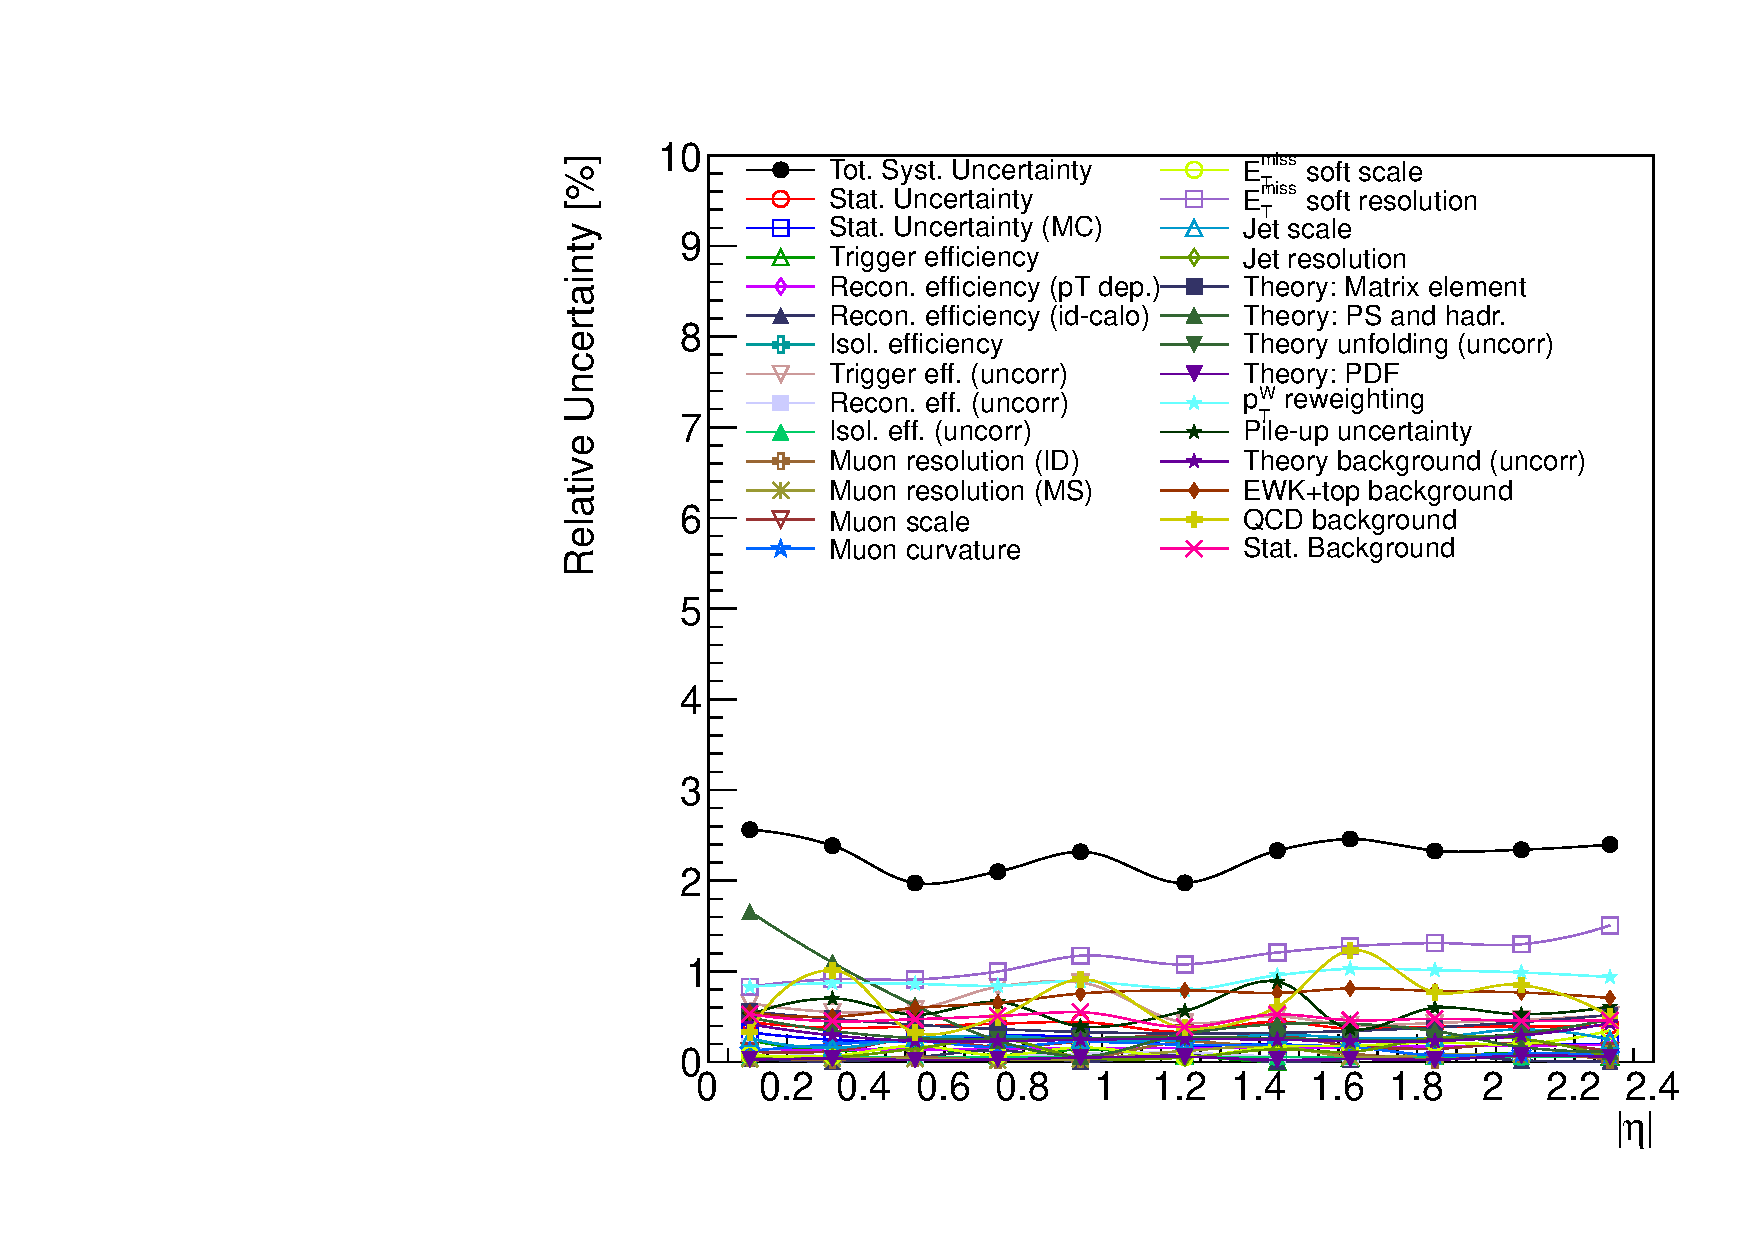
\includegraphics[width=0.32\textwidth]{/home/antonk/SupportingDocument/Wmunu/figures/res/Wmn_SYSTEM_2D_PT20_NEG_Unc_2d_Slice_2}
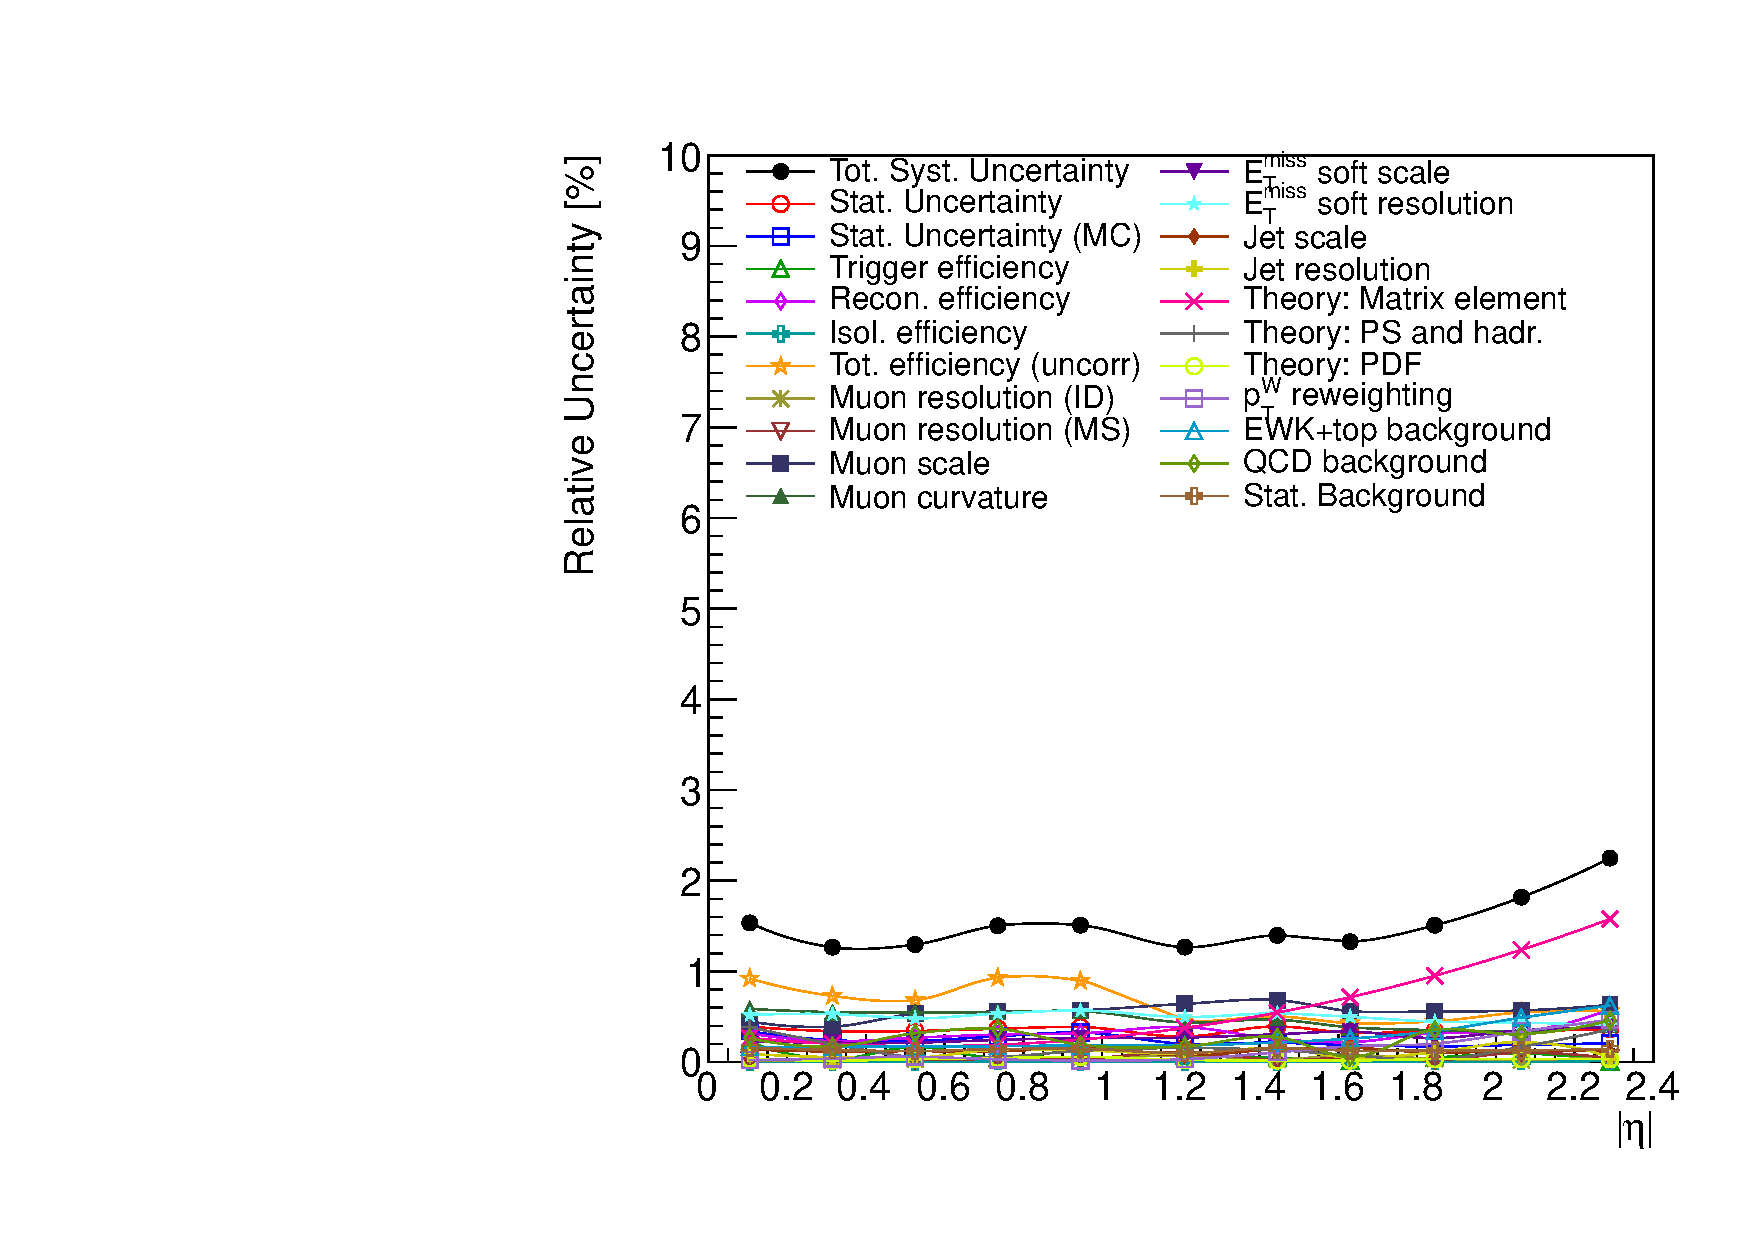
\includegraphics[width=0.32\textwidth]{/home/antonk/SupportingDocument/Wmunu/figures/res/Wmn_SYSTEM_2D_PT20_NEG_Unc_2d_Slice_5}

Representative uncertainties for \red{$W^+$}: $p_{T}>25$, $25<p_{T}<30$, $40<p_{T}<45$
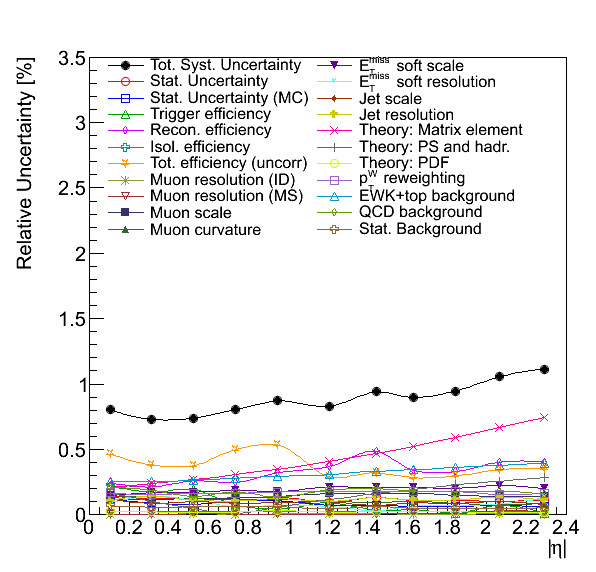
\includegraphics[width=0.32\textwidth]{/home/antonk/SupportingDocument/Wmunu/figures/res/Wmn_SYSTEM_1D_PT25_POS_Unc_proj}
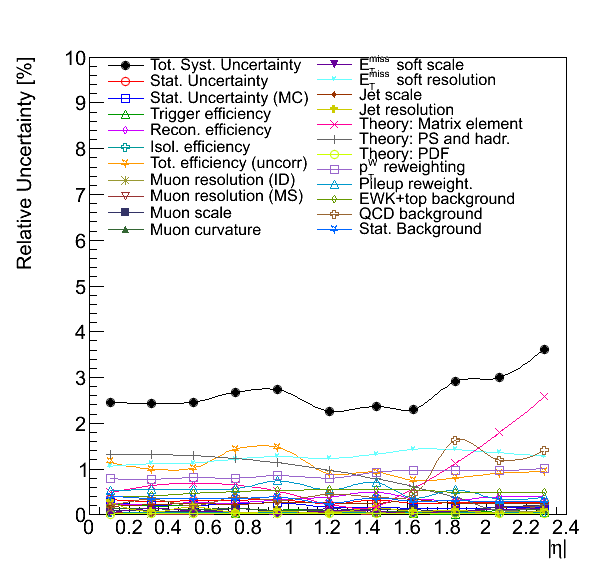
\includegraphics[width=0.32\textwidth]{/home/antonk/SupportingDocument/Wmunu/figures/res/Wmn_SYSTEM_2D_PT20_POS_Unc_2d_Slice_2}
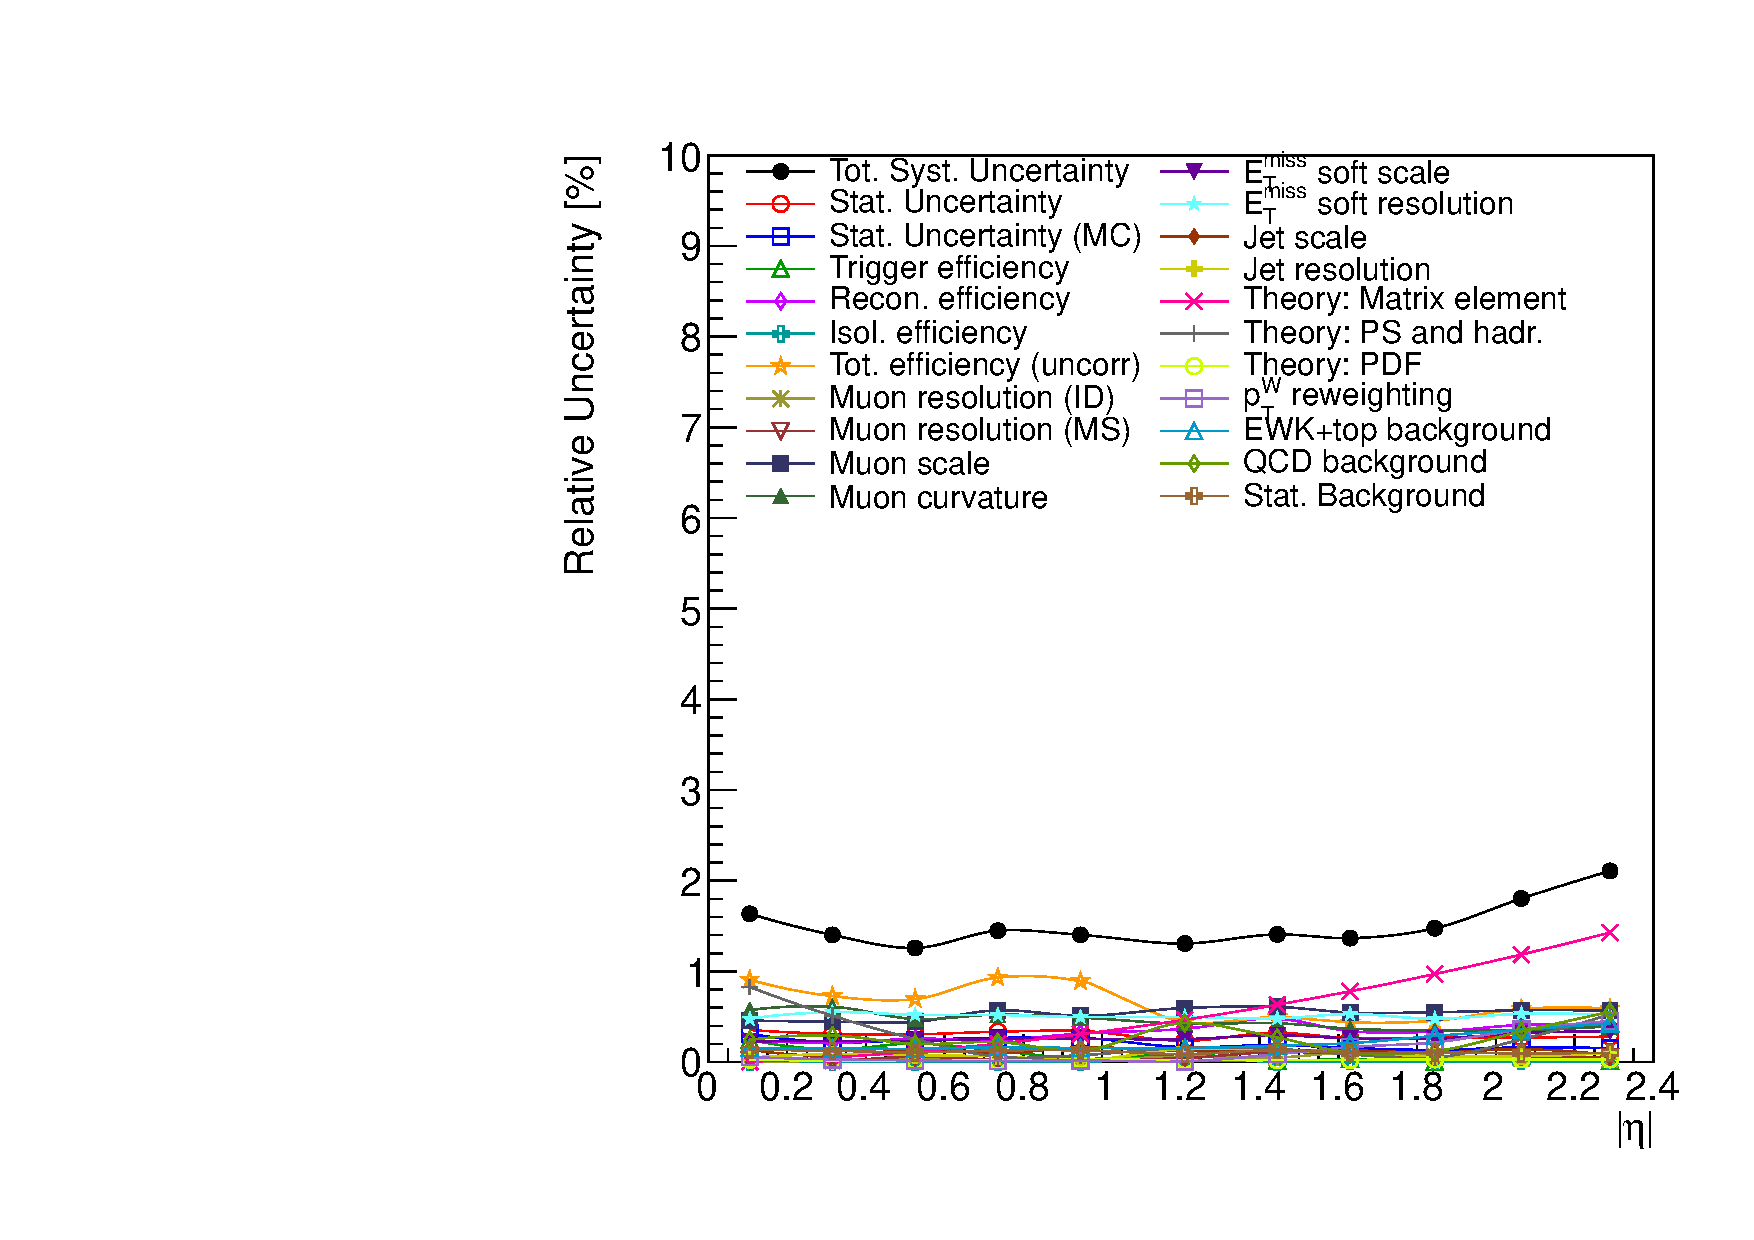
\includegraphics[width=0.32\textwidth]{/home/antonk/SupportingDocument/Wmunu/figures/res/Wmn_SYSTEM_2D_PT20_POS_Unc_2d_Slice_5}

}

\slide{Results: integrated cross-section }
{
\footnotesize{
Fiducial cross-sections:
$$\sigma^{fid}_{W^+}\cdot BR(W \rightarrow \mu\nu) = 2838.6 \pm 1.0 (\text{stat}) \pm 17.0 (\text{syst}) \pm 51.1 (\text{lumi})\ (pb)$$
$$\sigma^{fid}_{W^-}\cdot BR(W \rightarrow \mu\nu) = 1901.3 \pm 0.8 (\text{stat}) \pm 11.1 (\text{syst}) \pm 34.2 (\text{lumi})\ (pb)$$
Extrapolated to full phase space:
$$\sigma^{tot}_{W^+}\cdot BR(W \rightarrow \mu\nu) = 6327.3 \pm 2.5 (\text{stat}) \pm 107.8 (\text{syst}) \pm 113.9 (\text{lumi})\ (pb)$$
$$\sigma^{tot}_{W^-}\cdot BR(W \rightarrow \mu\nu) = 4351.6 \pm 2.1 (\text{stat}) \pm 98.1 (\text{syst}) \pm 78.3 (\text{lumi})\ (pb)$$
}

\centering
\small{NNLO predictions with NNPDF2.3, CT10, and ABM11 are best:}
\colb[T]
\column{.5\textwidth}
\centering
\includegraphics[width=0.85\textwidth]{/home/antonk/thesis/tex/res/fig/WpWm_ellipse}

\column{.5\textwidth}
\vspace{.1cm}
\centering
Correlated uncertainties (such as luminosity) cancel in the ratio:
\includegraphics[width=0.95\textwidth]{/home/antonk/thesis/tex/res/fig/WpWm_ratio}
\cole
}


\slide{Results: single-differential cross-section }
{

\small{NNLO predictions for $W^-$: HERAPDF1.5 and ABM11 are best.} \\
\small{NNLO predictions for $W^+$: HERAPDF1.5 and CT10 are best.}

\vspace{.2cm}
\colb[T]
\column{.5\textwidth}
\centering
$d\sigma/d|\eta_{\mu^{-}}|$
\includegraphics[width=0.95\textwidth]{/home/antonk/thesis/tex/res/fig/WMeta25_NNLO_combined}

\column{.5\textwidth}
\centering
$d\sigma/d|\eta_{\mu^{+}}|$
\includegraphics[width=0.95\textwidth]{/home/antonk/thesis/tex/res/fig/WPeta25_NNLO_combined}
\cole
}


\slide{Results: W charge asymmetry } 
{

\centering
$$A_{\mu} = \frac{d\sigma_{W^{+}}/d|\eta_{\mu^{+}}| - d\sigma_{W^{-}}/d|\eta_{\mu^{-}}|}{d\sigma_{W^{+}}/d|\eta_{\mu^{+}}| + d\sigma_{W^{-}}/d|\eta_{\mu^{-}}|}$$

\centering
\small{NNPDF2.3, followed by HERAPDF1.5 and CT10, provide best description. \\
MSTW2008 fails to describe the asymmetry:}

\centering
\includegraphics[width=0.45\textwidth]{/home/antonk/thesis/tex/res/fig/Wasym25_NNLO_combined}

}

\slide{Results: Double-differential $W^-$ cross-sections } 
{
	  \includegraphics[width=0.30\textwidth]{/home/antonk/thesis/tex/res/fig/WMetaPt25_30_NNLO_combined}
	  \includegraphics[width=0.30\textwidth]{/home/antonk/thesis/tex/res/fig/WMetaPt30_35_NNLO_combined}
	  \includegraphics[width=0.30\textwidth]{/home/antonk/thesis/tex/res/fig/WMetaPt35_40_NNLO_combined} \\
	  \includegraphics[width=0.30\textwidth]{/home/antonk/thesis/tex/res/fig/WMetaPt40_45_NNLO_combined}
	  \includegraphics[width=0.30\textwidth]{/home/antonk/thesis/tex/res/fig/WMetaPt45_50_NNLO_combined}
	  \includegraphics[width=0.30\textwidth]{/home/antonk/thesis/tex/res/fig/WMetaPt50_NNLO_combined}

\centering
\small{Data is between predictions of various PDF sets for $30<p_T<45$ GeV. At lower and higher values of $p_T$, PDFs undershoot the data (limitation of DYNNLO). }

}

\slide{Results: Double-differential $W^+$ cross-sections } 
{
	  \includegraphics[width=0.30\textwidth]{/home/antonk/thesis/tex/res/fig/WPetaPt25_30_NNLO_combined}
	  \includegraphics[width=0.30\textwidth]{/home/antonk/thesis/tex/res/fig/WPetaPt30_35_NNLO_combined}
	  \includegraphics[width=0.30\textwidth]{/home/antonk/thesis/tex/res/fig/WPetaPt35_40_NNLO_combined} \\
	  \includegraphics[width=0.30\textwidth]{/home/antonk/thesis/tex/res/fig/WPetaPt40_45_NNLO_combined}
	  \includegraphics[width=0.30\textwidth]{/home/antonk/thesis/tex/res/fig/WPetaPt45_50_NNLO_combined}
	  \includegraphics[width=0.30\textwidth]{/home/antonk/thesis/tex/res/fig/WPetaPt50_NNLO_combined}

\centering
\small{Data is between predictions of various PDF sets for $30<p_T<45$ GeV. At lower and higher values of $p_T$, PDFs undershoot the data (limitation of DYNNLO). }

}

\slide{Results: PDF fits } 
{
\iteb
\item Measurements in the \Wmn, \Wen, \Zmm, and \Zee\ channels are combined:
\iteb
\item $\chi^{2}/DOF$ of the combination: $54.68/53$
\itee
\item PDF fits via HERAFitter framework (HERA I + ATLAS data):
\iteb
\item $\chi^{2}/DOF \approx 13/11$
\itee
\itee

    \includegraphics[width=0.40\textwidth]{/home/antonk/thesis/tex/res/fig/pulls_104}
    \includegraphics[width=0.40\textwidth]{/home/antonk/thesis/tex/res/fig/pulls_105}

\footnotesize{Differential $d\sigma/d|\eta_{\ell^{-}}|$ (left) and $d\sigma/d|\eta_{\ell^{+}}|$ (right) cross-section measurement for $W \rightarrow \ell\nu$. The lower box shows the normalized data-theory pulls after the shifts of the correlated uncertainties (e.g., luminosity) are applied.}


}

\slide{Results: PDF sensitivity } 
{

Reduction of PDF uncertainty bands from ATLAS data:

\colb[T]
\column{.5\textwidth}
\includegraphics[width=0.92\textwidth]{/home/antonk/thesis/tex/QCD/figures/ZWu_dval_pdf_hess.pdf}\\
\includegraphics[width=0.92\textwidth]{/home/antonk/thesis/tex/QCD/figures/ZWu_uval_pdf_hess.pdf}

\column{.5\textwidth}
\centering

\includegraphics[width=0.92\textwidth]{/home/antonk/thesis/tex/QCD/figures/ZWu_s_pdf_hess.pdf}
\cole
}

\slide{Results: lepton universality } 
{

\iteb
\item Coupling of leptons to gauge bosons should be flavor-independent.
\item Probed by comparing (\Wmn\ and \Wen), (\Zmm\ and \Zee)
\item Better precision from W than the current world average!
\itee

\begin{figure}
  \begin{center}
    \includegraphics[width=0.55\textwidth]{/home/antonk/thesis/tex/res/fig/ZWluni_ellipse}
  \end{center}
\end{figure}

}

\slide{Conclusions}
{
\iteb
\item Measured integrated, single- and double-differential \Wmn\ cross-sections
\item Good understanding of the detector $\rightarrow$ sub-percent level of precision
\item Lepton universality confirmed to better-than-PDG precision
\item Existing PDF families provide various levels of agreement with the data
\iteb
\item Tensions are seen in some regions of phase space
\itee
\item Measurement allows to reduce PDF uncertainties, particularly for down and strange quarks
\iteb
\item Detailed PDF fit studies are still ongoing
\itee
\item Double-differential measurement is the first of its kind
\iteb
\item 2-4\% uncertainty in most $p_T$ slices
\item Disagreements with NNLO predictions away from Jacobian peak
\item Seen as a limitation of fixed-order QCD calculations
\itee
\itee
}

%%%%%%% Back-up slides %%%%%%%%%%
\appendix
\newcounter{finalframe}
\setcounter{finalframe}{\value{framenumber}}

\slide{}
{
\centering
\Huge Back-up slides
}


\slide{ATLAS Sensitivity region}
{
 \begin{columns}
  \begin{column}{0.5\textwidth}
    \vskip-3ex
    \begin{small}
      \begin{itemize}
        \item W,Z data cover a $x, Q^2$ kinematic range given by the
          boson masses $M_{W,Z}$, $E_p = 3.5$ TeV and $|y_{W,Z}| < 3.6$
        \item Corresponds to $Q^2 = M_{W,Z}^2$ and $0.001 < x <0.1$
        \item Maximal sensitivity at central rapidity, $y_Z = 0$,
          corresponds to $x = M_Z/2 \cdot E_p \sim 0.013$
        \item $x=0.013$ at $Q^2= M_Z^2$ $\rightarrow$ $x=0.023$ at $Q^2=1.7~\rm{} GeV^2$
          (Due to gluon radiation via QCD evolution)
      \end{itemize}
    \end{small}
  \end{column}
  \begin{column}{0.5\textwidth}
    \begin{center}
      \begin{figure}
        \includegraphics[width=\textwidth]{/home/antonk/SupportingDocument/talk/PDFfit/figures/atlas_xq}
      \end{figure}
      \vskip-2ex
  \end{center}
 \end{column}
\end{columns}
}


\slide{QCD fits framework}
{
 \begin{columns}
  \begin{column}{0.5\textwidth}
    \vskip-3ex
    \begin{small}
      \begin{itemize}
      \item PDFs are extracted through QCD Fit analysis
      \item Open source HERAFitter framework
        \link{http://www.herafitter.org/HERAFitter}{http://www.herafitter.org/HERAFitter}
      \item Fits performed at NNLO, using general mass
        variable flavour scheme
        \item Theoretical ingredients
      \begin{itemize}
      \item W, Z cross sections calculated with
        APPLGRID interfaced to MCFM at NLO QCD
      \item NNLO/NLO k-factors calculated with DYNNLO and FEWZ
      \item NLO EW corrections calculated with FEWZ and SANC
      \end{itemize}
      \end{itemize}
    \end{small}
  \end{column}
  \begin{column}{0.5\textwidth}
   \vskip-3ex
   Input data
   \begin{itemize}
   \item{ATLAS W,Z 2011: 5 datasets after electron-muon-CF combination}
     \begin{itemize}
     \item{$Z$ low mass (46-66)}
     \item{$Z$ central mass (66-116)}
     \item{$Z$ high mass (116-150)}
     \item{$W^+ \rightarrow l^+ \nu$}
     \item{$W^- \rightarrow l^- \nu$}
     \end{itemize}
   \item HERA I $e\pm p$ NC, CC
   \end{itemize}
  \end{column}
 \end{columns}
}



\slide{MC re-weightings}
{

\begin{itemize}
\item Multiple MC small deficits \raw\ reweighting, derived from
\begin{itemize}
\item data/MC comparisons at the reconstructed level
\item comparisons of different MC samples at truth level\\ (e.g. when a MC has a known deficit)
\item  using information from other ATLAS measurements 
\end{itemize}
\item Weights applied at the truth level and validated at the reco level 
\end{itemize}

\scriptsize 

\renewcommand{\arraystretch}{1.3}

\begin{block}{Reweightings}
\begin{tabular}{ll}
\textbf{Pileup}               & vs. $\mu$ to equalise the amount of pileup in data and MC \\

\textbf{Vertex Spread in $z$} & to match the spread of the beam spot in $z$ direction.\\
& Crucial to control lepton ID performance at the permille level \\

\textbf{$W$ and $Z$ Boson $p_T$} & reweighted to alternative samples, as motivated by ATLAS
                                               $Z$ $\phi^*$, $\pt$ \\
& and $W$ $\pt$ analyses and data\\

\textbf{$W$ and $Z$ Boson Line Shape} & Nearly all MCs with slightly different electroweak 
                                                    setup ($m_V$, $\Gamma_V$, $\alpha_{em}$). \\ 
&                                                    Reweight all MCs to the same 
                                                    \textit{Improved Born Approximation} definition \\

\textbf{PDF} & To study systematics due to PDF uncertainties \\

\textbf{\Alpgen\Herwig\ Boson Rapidity} & To fix rapidity spectrum of 
                                                      \Alpgen\Herwig\ $W\to\tau\nu$, $\Zg\to\tau\tau$ \\
\textbf{Polarisation and Ang. Coeff.} &  For testing purposes to understand better differences between MCs\\
\end{tabular}
\end{block}

}


\slide{Data samples}
{

\begin{table}[p]
  \tiny
  \begin{center}
    \begin{tabular}{l|l|r|r}
      \hline
      \hline
      \raisebox{-0.4ex}{Process} & Generator & $\sigma{\cdot}
      \text{BR}{\cdot}\epsilon_{filter}$ [nb] & $N_{evt}\,[10^6]$\\
      \hline\hline

      \multicolumn{3}{c}{Signal samples for \Wln}\\\hline
      \Wplusmunu     &  \Powheg\Pythia  & 6.16 (5\%) & 23 \\
      \Wminusmunu    &  \Powheg\Pythia  & 4.30 (5\%) & 17 \\
      \Wplusmunu     & \Powheg\Herwig   & 6.16 (5\%) & 16 \\
      \Wminusmunu    & \Powheg\Herwig   & 4.30 (5\%) & 12 \\
      \Wplusmunu     & \Mcatnlo & 6.16 (5\%) & 16 \\
      \Wminusmunu    & \Mcatnlo & 4.30 (5\%) & 12 \\

      \hline \multicolumn{3}{c}{\Zgll\ samples}\\\hline
      \Zgll ~~($\mll > 53.8\gev$) &   \Powheg\Pythia   &  1.01 (5\%) & 20\\
      \Zgll ~~($\mll < 53.8\gev$)  &  \Powheg\Pythia   &  0.088 (5\%) & 3\\

      \hline \multicolumn{3}{c}{\Alpgen\Herwig\  and \Sherpa\ \Wln\ and \Zgll\ samples}\\\hline
      \Wtau\ Np0   &   \Alpgen\Herwig\ & 8.29 (5\%) & 3.4 \\
      \Wtau\ Np1   &   \Alpgen\Herwig\ & 1.56 (5\%) & 2.5 \\
      \Wtau\ Np2   &   \Alpgen\Herwig\ & 0.45 (5\%) & 3.8 \\
      \Wtau\ Np3   &   \Alpgen\Herwig\ & 0.12 (5\%) & 1 \\
      \Wtau\ Np4   &   \Alpgen\Herwig\ & 0.03 (5\%) & 0.25 \\
      \Wtau\ Np5   &   \Alpgen\Herwig\ & 0.008 (5\%) & 0.07 \\

      \Ztau\ Np0  &  \Alpgen\Herwig\  & 0.83 (5\%) & 6.6 \\
      \Ztau\ Np1  &  \Alpgen\Herwig\  & 0.17 (5\%) & 1.3 \\
      \Ztau\ Np2  &  \Alpgen\Herwig\  & 0.051 (5\%) & 0.81 \\
      \Ztau\ Np3  &  \Alpgen\Herwig\  & 0.014 (5\%) & 0.22 \\
      \Ztau\ Np4  &  \Alpgen\Herwig\  & 0.004 (5\%) & 0.06 \\
      \Ztau\ Np5  &  \Alpgen\Herwig\  & 0.0009 (5\%) & 0.02 \\

      \hline \multicolumn{3}{c}{$t\bar{t}$ and single top samples}\\\hline
      $t\bar{t}$   & \Mcatnlo & 0.098 (6.2\%) & 1.5\\
      single top, $t$ chan  & \Mcatnlo & $7.12\cdot 10^{-3}$ (12\%) & 0.3\\
      single top, $s$ chan & \Mcatnlo & $0.47\cdot 10^{-3}$ (12\%) & 0.3\\
      single top, $Wt$ chan & \Mcatnlo & $14.59\cdot 10^{-3}$ (12\%) & 0.9\\

      \hline \multicolumn{3}{c}{Diboson samples}\\\hline
      $WW$ & \Herwig & 17.5 $\cdot 10^{-3}$ (7\%) & 1.5 \\
      $WZ$ & \Herwig & 5.7 $\cdot 10^{-3}$ (7\%) & 1 \\
      $ZZ$ & \Herwig & 1.3 $\cdot 10^{-3}$ (7\%) & 0.25 \\

      \hline \multicolumn{3}{c}{QCD samples (for cross-checks only)}\\\hline
      $b\overline{b}$ ($p_{T, \mu} > 15\gev$) & \Pythia & $73.9$ & 4.5\\
      $c\overline{c}$ ($p_{T, \mu} > 15\gev$) & \Pythia & $28.4$ & 1.5\\

      \hline\hline
    \end{tabular}
    \caption{ Monte-Carlo samples used in the analysis. The numbers in the parentheses next to cross-section values indicate the uncertainty on these cross-sections. The quoted cross-sections are the ones used to normalize the estimates of expected Monte-Carlo event counts. }
    \label{tab:samples}
  \end{center}
\end{table}

}


\slide{Muon momentum corrections }
{

\begin{itemize}

\item Using standard MCP recommendation with one exception:
\begin{itemize}
\item muon momentum scale re-derived using full-2011 statistics (but same method)
\end{itemize}

\item Momentum Scale
\begin{itemize}
\item Two corrections from \Zmm\ events: overall scale (``K'') based on peak position 
and curvature (``C'') balancing $\mu^+$ and $\mu^-$ in data
\item Derived in $\eta$ regions: \{$0-1.05$, $1.05-1.7$, $1.7-2.0$, $2.0-2.5$\} (A,C sides) 
  $$K \equiv \frac{M_{Z}^{data}}{M_{Z}^{MC}} \approx \frac{p_{T}^{measured}}{p_{T}^{corrected}}~~~~~
  \frac{1}{p_{T}^{corrected}} \equiv \frac{1}{p_{T}^{measured}} + (q \cdot C)$$
\item K in $0.1-0.5\%$ range, C in $10-200\cdot 10^{-6}\,GeV$ (eg. $\Delta p_T/p_T=0.1/20$, in GeV)
\item Small corrections known with 10-50\% precision \raw\ small impact in most cases
\end{itemize}

\item Momentum Resolution
\begin{itemize}
\item From template fits of $m_{\mu\mu}$ in \Zmm\ events and MS-to-ID curvature difference weighted 
by the electric charge %$(\frac{Q}{p_{T}^{ID}}-\frac{Q}{p_T^{MS}})$ 
(for both \Zmm\ and \Wmn\ events) in the same $\eta$ regions as above
\item Multiple scattering and intrinsic resolution MS corr. in $1.8-5.2\%$ and $0.2-0.3\,TeV^{-1}$, respectively.
The ID intrinsic resolution corr. in $0.2-0.5\,TeV^{-1}$ (no correction for multiple scattering)
\item Very small corrections known with 20-40\% precision \raw\ very small impact
\end{itemize}

\end{itemize}

}


\newcommand{\CaloIso}{\ensuremath{\mathtt{Iso98}E_{T}^\mathrm{cone20}}}
\newcommand{\TrackIso}{\ensuremath{\mathtt{Iso97}p_{T}^\mathrm{cone40}}}
\newcommand{\TrackIsoMu}{\ensuremath{\sum p_T^{\mathrm{cone40}}/p_{T}<0.1}}

\slide{Reconstruction efficiency SFs}
{

\begin{itemize}
\item Very similar to default MCP SFs, but custom binning
\item Computed on a per-period basis
\item Nominal binning: 2D+charge ($\eta,\phi,q$), in bins of measurement
\item Systematic uncertainty
\begin{itemize}
\item Driven by the difference between ID-only and CaloTag muon probes
\item Typical uncertainty: 0.2-0.3\%
\end{itemize}
\end{itemize}

\vspace{-0.5cm}

\begin{figure}
  \centering
  \subfloat[Nominal SFs]{\includegraphics[width=0.45\textwidth]{/home/antonk/thesis/tex/MuonPerformance/figures/NewRecoSF/SF_etaPhi_negq}}
  \subfloat[CaloTag-ID probe]{\includegraphics[width=0.45\textwidth,angle=0]{/home/antonk/thesis/tex/MuonPerformance/figures/NewRecoSF/CaloDeviation_etaPhi_negq}}
\end{figure}

}

\slide{Isolation efficiency SFs}
{
\begin{itemize}
\item Track-based isolation: \TrackIsoMu
\item SFs binned vs $p_T$, since they were found flat vs other variables
\item Systematic uncertainty
\begin{itemize}
\item Estimated by varying Z TB selection cuts by $\pm10\%$
\item Statistically significant shifts are added in quadrature
\item Typical uncertainty: $\leq 0.1\%$
\end{itemize}

\end{itemize}

\vspace{-0.5cm}

\begin{figure}
  \centering
  \subfloat[\tiny \TrackIsoMu\ SF vs $\eta$]{\includegraphics[width=0.33\textwidth]{/home/antonk/thesis/tex/MuonPerformance/figures/eff_cb_isoid40rel01_mu_probe_eta}}
  \subfloat[\tiny \TrackIsoMu\ SF vs $p_T$]{\includegraphics[width=0.33\textwidth,angle=0]{/home/antonk/thesis/tex/MuonPerformance/figures/eff_cb_isoid40rel01_mu_probe_pt}}
  \subfloat[\tiny \TrackIsoMu\ SF vs $<\mu>$]{\includegraphics[width=0.33\textwidth,angle=0]{/home/antonk/thesis/tex/MuonPerformance/figures/eff_cb_isoid40rel01_mu}}
\end{figure}

}

%===========================================
%  Slide -1
%===========================================

\slide{Trigger efficiency SFs}
{

\begin{itemize}
\item Single-muon \texttt{MuId} trigger (\texttt{mu18} and \texttt{mu18\_medium})
\item Customized version of muon trigger group SFs (binning, higher MC stats)
\item Nominal binning: 2D+charge ($\eta,p_T,q$), in bins of measurement
\item Systematic uncertainty
\begin{itemize}
\item Previously dominant $q$, $p_T$ dependence effects no longer apply
\item Remaining systematic: adding residual $\phi$ corrections on top of nominal SFs
\item Typical uncertainty: 0.1-0.3\%
\end{itemize}
\end{itemize}

\vspace{-0.5cm}

\begin{figure}
  \centering
  \subfloat[Trigger SFs: G-I]{\includegraphics[width=0.5\textwidth]{/home/antonk/thesis/tex/MuonPerformance/figures/scaleFactors/mu18_neg_SF_eta_pt}}
  \subfloat[Trigger SFs: L3-L4 (RPC problems)]{\includegraphics[width=0.5\textwidth,angle=0]{/home/antonk/thesis/tex/MuonPerformance/figures/scaleFactors/rpc_pos_SF_eta_pt}}
\end{figure}

}


% Pathological bin
\begin{frame}{Perf. issue: Muon Trigger /1}

\begin{itemize}
\item A pathological bin shown here
\item The effect is present only after the technical stop!
\end{itemize}

\vspace{-0.5cm}

\centering

\begin{figure}[phtb]
  \subfloat[\tiny W, $\mu^-$, $1.95<|\eta|<2.18$, C-side]{%
    \includegraphics[width=0.25\textwidth]{/home/antonk/thesis/tex/Wmunu/figures/AC/eta/W_10_C_stack_l_eta_NEG}
  }
  \subfloat[\tiny W, $\mu^-$, $1.95<|\eta|<2.18$, A-side]{%
    \includegraphics[width=0.25\textwidth]{/home/antonk/thesis/tex/Wmunu/figures/AC/eta/W_10_A_stack_l_eta_NEG}
  } \\
  \subfloat[\tiny Z, $\mu^-$, $1.95<|\eta|<2.18$, C-side]{%
    \includegraphics[width=0.25\textwidth]{/home/antonk/thesis/tex/Wmunu/figures/AC/eta/Z_10_C_stack_lN_eta_ALL}
  }
  \subfloat[\tiny Z, $\mu^-$, $1.95<|\eta|<2.18$, A-side]{%
    \includegraphics[width=0.25\textwidth]{/home/antonk/thesis/tex/Wmunu/figures/AC/eta/Z_10_A_stack_lN_eta_ALL}
  }
 %% \caption{\it $\mu^-$ $\eta$ distributions for W and Z candidates inside the 10th $|\eta|$ bin ($1.95<|\eta|<2.18$). A dip is seen on the C-side, but only in W events.}
 %% \label{fig:Wmunu:AC_eta_NEG_10}
\end{figure}

\end{frame}

%===========================================
%  Slide -1
%===========================================

\begin{frame}{Perf. issue: Muon Trigger /2}

\begin{itemize}
\item The effect is not present with the \texttt{MuId} trigger chain (on the right)
\item Moreover, the effect cannot be corrected with TB due to a bug in trigger matching!
\end{itemize}

\begin{figure}[phtb]
  \begin{center}
        \subfloat[\texttt{MG} chain: \Wminus, $1.95<|\eta|<2.18$, C-side]{%
	  \includegraphics[width=0.5\textwidth]{/home/antonk/thesis/tex/Wmunu/figures/AC/old/WMU18_MG_10_C_stack_l_eta_NEG}
        }
        \subfloat[\texttt{MuId} chain: \Wminus, $1.95<|\eta|<2.18$, C-side]{%
	  \includegraphics[width=0.5\textwidth]{/home/antonk/thesis/tex/Wmunu/figures/AC/old/WMU18_10_C_stack_l_eta_NEG}
        }
 %% \caption{\it Efficiency dips seen in W but not Z events are only present with the muGirl triggers (mu18\_MG and mu18\_MG\_medium). They disappear when muid triggers are used (mu18 and mu18\_medium). Here, this is shown explicitly for \Wminus\ events in the $1.95<|\eta|<2.18$ bin. }
 %% \label{fig:Wmunu:AC_mu18_NEG_10}
 \end{center}
\end{figure}

\end{frame}

% UNFOLDING
%===========================================
%  Slide Unfolding
%===========================================

\slide{Unfolding details}
{
\iteb
\item Migrations in rapidity ($\eta_\ell$, $y_Z$) are negligible:
 essentially only an efficiency correction
\item Migrations in mass $m_{\ell\ell}$ and lepton $p_T$ are larger.
Each channel studied Bayesian vs bin-by-bin options and concluded that bin-by-bin is fine.
\itee

%% W
\only<1>{

\colb[t]
\column{.5\textwidth}

\centering
\scriptsize{Purity  for \Wplusmn \\ fraction of reconstructed events \\generated in same bin}
\includegraphics[width=0.8\textwidth]{/home/antonk/thesis/tex/Wmunu/figures/purity/purity_2D_pos}

\column{.5\textwidth}

\centering
\scriptsize{Purity  for \Wminusmn \\ fraction of reconstructed events \\generated in same bin}
\includegraphics[width=0.8\textwidth]{/home/antonk/thesis/tex/Wmunu/figures/purity/purity_2D_neg}

\cole

}

\only<2>{

\colb[t]
\column{.5\textwidth}

\centering
\scriptsize{Percent deviations wrt. bin-by-bin \\for \Wplusmn\ ($1.37<\eta<1.52$)}
\includegraphics[width=0.8\textwidth]{/home/antonk/thesis/tex/Wmunu/figures/res/Wmn_UNFTST_2D_PT20_POS_unfIte_2d_Slice_7_proj}

\column{.5\textwidth}

\centering
\scriptsize{Percent stat. uncert. increase wrt. bin-by-bin \\for \Wplusmn\ ($1.37<\eta<1.52$)}
\includegraphics[width=0.8\textwidth]{/home/antonk/thesis/tex/Wmunu/figures/res/Wmn_UNCTST_2D_PT20_POS_statUnfIte_2d_Slice_7_proj}

\cole

}

}


% UNCERTAINTIES

\slide{Multi-jet background uncertainties in \Wmn}
{

\centering

\includegraphics[width=0.39\textwidth]{/home/antonk/SupportingDocument/Wmunu/figures/qcdunc/Q0_qcd_ptALL25_etaLOOP_syst_rel_bgsub}
\includegraphics[width=0.39\textwidth]{/home/antonk/SupportingDocument/Wmunu/figures/qcdunc/Q1_qcd_ptALL25_etaLOOP_syst_rel_bgsub}

\vspace{-0.33cm}

\includegraphics[width=0.39\textwidth]{/home/antonk/SupportingDocument/Wmunu/figures/qcdunc/Q0_qcd_pt2_etaLOOP_syst_rel_bgsub}
\includegraphics[width=0.39\textwidth]{/home/antonk/SupportingDocument/Wmunu/figures/qcdunc/Q0_qcd_pt7_etaLOOP_syst_rel_bgsub}

}


% COMB

\slide{Combination across channels}
{

\begin{table}[htbp]   
\tiny
  \begin{center}
    \begin{tabular}{lccccc}
      \hline
      \hline
      & \multicolumn{5}{c}{Channel} \\
      Uncertainty Source & \Wen\ & \Zee\ & \Zee\ (CF) & \Wmn\ & \Zmm\  \\
      \hline
      \input{/home/antonk/thesis/tex/tables/systematic_correlations.tex}
      \hline
      \hline
    \end{tabular}
  \end{center}
    \caption{Summary of the correlations for the uncertainties.}
    \label{tab:SystCorr}
\end{table}

}
